\documentclass[10pt]{article}

% PREAMBULE -------------------------------------------------------------------------
% 
% If you want to edit the text please scroll down to the CONTENT
% 
% This document is written in LaTeX
% For quick doc please follow to http://web.mit.edu/olh/Latex/ess:Latex.html
% All used symbols may be found here: http://www.artofproblemsolving.com/Wiki/index.php/LaTeX:Symbols
% Graphz are using the TikZ package: http://texamples.net/tikz

\usepackage{fullpage, url, tikz, tikz-er2, listings, sidecap, floatrow}
\usepackage{graphicx}
% TikZ is included in the TeXLive distribution
% TikZ-ER2 (Creative Commons Attribution 2.5 Generic License) 
% needs to be installed https://www.assembla.com/wiki/show/tikz-er2 

\DeclareGraphicsExtensions{.pdf,.png,.jpg}

\def\Ua{{\tt Ua}}
\def\Ub{{\tt Ub}}
\def\La{{\tt La}}
\def\Ma{{\tt Ma}}
\def\Mb{{\tt Mb}}

\def\xpi{{\tt XPI}}
\def\amo{{\tt AMO}}

\def\headsto{${\Longrightarrow}$ }
\def\hto{\headsto}
\def\eq{${\supset}$ }

\def\version{alpha 0.1}

\usetikzlibrary{positioning}
\usetikzlibrary{shadows}

\tikzstyle{every entity} = [top color=white, bottom color=blue!30, 
                            draw=blue!50!black!100, drop shadow, rounded corners]
\tikzstyle{every weak entity} = [drop shadow={shadow xshift=.7ex, 
                                 shadow yshift=-.7ex}, rounded corners]
\tikzstyle{every attribute} = [top color=white, bottom color=yellow!20, 
                               draw=yellow, node distance=1cm, drop shadow, rounded corners]
\tikzstyle{every relationship} = [top color=white, bottom color=red!20, minimum size=2.3cm,
                                  draw=red!50!black!100, drop shadow, rounded corners]
\tikzstyle{every isa} = [top color=white, bottom color=green!20, 
                         draw=green!50!black!100, drop shadow, rounded corners]
                         
% CONTENT -----------------------------------------------------------------------------                         
                         
\title{Mozilla Addon Builder\\ Package Building System}
\author{Piotr Zalewa}
\date{\today, \version}

\begin{document}
\maketitle

{\scriptsize
	\noindent Download this document from \\
\url{http://github.com/zalun/FlightDeck/raw/master/Docs/Package%20Building\%20System.pdf}\\
}{\scriptsize
	\noindent If in doubts, please take a look at the accompanied slides at \\
	\url{http://github.com/zalun/FlightDeck/raw/master/Docs/Addon\%20Builder\%20-\%20Build\%20System.pdf}
}

\section{Assumptions for the current iteration}

	\begin{enumerate}
		\item{Name of the Package is not unique anymore.\\
			Packages are identified by it's {\em unique ID}. There may and probably often will be many
			Packages with the same name\footnote{Check if it will not make any problem with Addons and 
			uploading to \amo}.\\
			{\tt /library/123456/}}
		\item{Version is a tag.\\
			Version is important. It is used to tag major {\em Revisions}. If a package is called without any
			Version specified, the latest versioned Revision will be used.\\
			{\tt /library/123456/version/0.1/}}
		\item{Revision Number is used to precisely identify a Revision.\\
			It is completely parallel to the Package Version\\
			{\tt /library/123456/revision/654/}}
		\item{No collaborative editing.\\
			That means there is no connection between Packages owned by different Users.}
		\item{Package remembers wich SDK version was used to build it.\\
			This is very complicated also on the front-end side. It will be created during the next
			iteration.}
	\end{enumerate}

\section{Logical structure}

	\scalebox{1}{\begin{tikzpicture}[node distance=1cm, every edge/.style={link}]
		\node [entity] (User) {User};
		\node [entity] [right=of User] (Package) {Package} edge [->] (User)
			node [attribute] [above=of Package] {ID} edge (Package);
		\node [entity] [right=1.5cm of Package] (PackageRevision) {PackageRevision} edge [->] (Package)
			node [attribute] [below=of PackageRevision] {Version} edge [dashed] (PackageRevision)
			node [attribute] (meta) [below left=6mm of PackageRevision] {Meta} edge (PackageRevision)
				node [attribute] [below=of meta] {Name} edge (meta)
				node [attribute] [below left=of meta] {Description} edge (meta);
		\node [relationship] [above=1.5cm of PackageRevision] (depends) {depends on};
		\draw
			(PackageRevision.60) edge [<-] (depends.320) 
			(PackageRevision.130) edge node [rectangle,fill=white,rotate=277] {Library} (depends.220);
		\node [entity] [right=of PackageRevision] (Module) {Module} edge [total] (PackageRevision)
			node [attribute] [right=of Module] {Code} edge (Module);
		\node [entity] [below=of Module] (Attachment) {Attachment} 	edge [total] (PackageRevision)
			node [attribute] [right=of Attachment] {Filename} edge (Attachment);		
	\end{tikzpicture}}


\section{Exporting \xpi}

	Be aware that it is possible and common to export \xpi\footnote{An \xpi\ (pronounced "zippy" and derived 
	from XPInstall) installer module is a ZIP file that contains an install script or a manifest at the root 
	of the file, and a number of data files.} from partially unsaved data. This happens when User will use 
	the "Try in browser" 	functionality. In this case \xpi\ may not be send to 
	\amo\footnote{\url{http://addons.mozilla.org/}}.
	
	\subsection{Creating directory structure}
		
		Directory structure should be as close as standard Jetpack SDK as possible. 
		
		\subsubsection*{Copy Jetpack SDK to a temporary dir}
		
			\begin{lstlisting}
/tmp/jetpack-sdk-
|-- bin
|   |-- activate
|   |-- bin
|   `-- [...]
|-- packages
|   |-- development-mode
|   |-- jetpack-core
|   |-- nsjetpack
|   `-- test-harness
|-- python-lib
|-- static-files
`-- [...]
			\end{lstlisting}
		
	\subsection{Exporting Packages with Modules}
		
		\begin{enumerate}
			\item{Create Package and its Modules directories\\
				{\tt /tmp/packages\_\{hash\}/\{Package:name\}/}\\
				{\tt /tmp/packages\_\{hash\}/\{Package:name\}/lib/}
			}
			\item{Use collected data to create the Manifest.\\
				{\tt /tmp/packages\_\{hash\}/\{Package:name\}/package.json}
			}
			\item{Create Module files\\
				Iterate over the assigned Modules and create a "{\tt .js}" file with its content inside 
				Package's {\tt lib/} directory.
			}
			\item{Export dependencies\\
				Iterate over Libraries on which a Package depends and repeat this section ({\em Export 
				the Package with Modules}) for every Library.
			}
		\end{enumerate}
	
	\subsection{Building \xpi}
	
		System is already in a virtual environment knowing about Jetpack SDK. It is enough to change 
		directory to {\tt /tmp/packages\_\{hash\}/\{Package:name\}/} and call {\tt cfx xpi}. The 
		{\tt \{Package:name\}.xpi} file will be created in current directory. Its location is then send
		to the front-end to be used in further actions, usually calling the {\em FlightDeck Addon}\footnote{
		FlightDeck Addon is a Jetpack extension allowing to temporary installation of the \xpi. It 
		needs to be called with an URL of the \xpi.} to download and install the \xpi.
	
	\subsection{Uploading to AMO}
	
		Create \xpi\ from the database object. Use {\tt mechanize} lib to login to \amo and upload the 
		file faking it was done directly from the browser.
							
\section{Editing Package and its Modules}

	How database evolves by changing the Packages and Modules. This description will be used later to design 
	structure and functionalities of the system.

	\subsection{Starting point}
		\noindent All next scenarios start from the {\tt Ua:La.1} defined as below.
		\subsubsection*{{\tt La \hto  Ua:La.1 \eq \{Ua:La.1:Ma\}}}
			Package \La\ is created by User \Ua.\\
			\La's HEAD is PackageRevision identified as {\tt Ua:La.1}\\
			It contains only one module - \Ma
			
			\noindent Following steps had to happen to achieve above status:

			\vspace{5mm}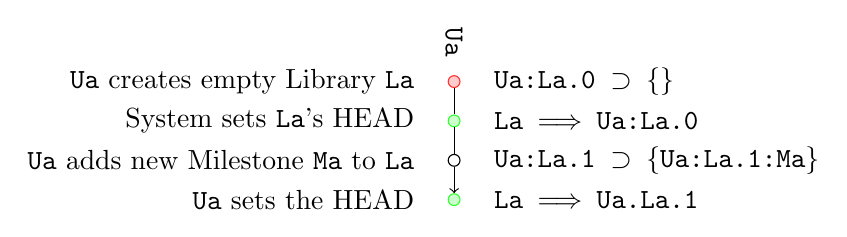
\begin{tikzpicture}[
				save/.style={circle,draw,minimum size=1.5mm},
				branch/.style={circle,draw=red!80,fill=red!20,minimum size=1.5mm},
				heads/.style={circle,draw=green!80,fill=green!20,minimum size=1.5mm},
				branchfrom/.style={circle},
				labr/.style={anchor=west,font=\tt},
				labl/.style={anchor=east},
				bend angle=45,
				inner sep=0pt]
				\node at (0,5mm) [rotate=270] {\Ua};
				\node [branch] 		(UaLa0) 		at (0,0)				{}
					node [labr] at (5mm,0) 	{Ua:La.0 \eq \{\}}
					node [labl] at (-5mm,0)	{\Ua\ creates empty Library \La};
				\node [heads]		(LaUaLa0)		at (0,-5mm)			{}
					edge (UaLa0)
					node [labr] at (5mm,-5mm)	{La \hto Ua:La.0}
					node [labl] at (-5mm,-5mm)	{System sets \La's HEAD};
				\node [save]		(UaLa1)		at (0,-10mm)			{}
					edge (LaUaLa0)
					node [labr] at (5mm,-10mm)	{Ua:La.1 \eq \{Ua:La.1:Ma\}}
					node [labl] at (-5mm,-10mm)	{\Ua\ adds new Milestone \Ma\ to \La};
				\node [heads]		(LaUaLa1)		at (0,-15mm)			{}
					edge [<-] (UaLa1)
					node [labr] at (5mm,-15mm) 	{La \hto Ua.La.1}
					node [labl] at (-5mm,-15mm)	{\Ua\ sets the HEAD};
			\end{tikzpicture}
			
	\subsection{Scenario (1 Module, 2 Users, no dependencies)}
		\Ua\ and \Ub\ are working on \La\\
		\Ub\ modified one module

		\vspace{3mm}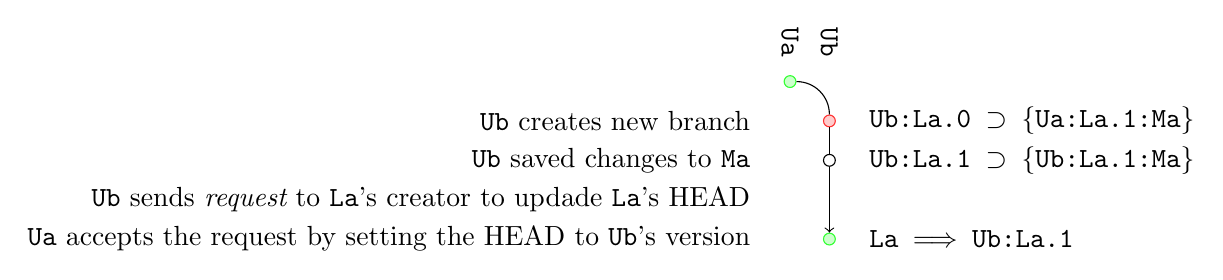
\begin{tikzpicture}[
			save/.style={circle,draw,minimum size=1.5mm},
			branch/.style={circle,draw=red!80,fill=red!20,minimum size=1.5mm},
			heads/.style={circle,draw=green!80,fill=green!20,minimum size=1.5mm},
			branchfrom/.style={circle},
			labr/.style={anchor=west,font=\tt},
			labl/.style={anchor=east},
			bend angle=45,
			inner sep=0pt]
			\node at (0,5mm) [rotate=270] {\Ua};\node at (5mm,5mm) [rotate=270] {\Ub};
			\node [heads] 		(UaLa1) 		at (0,0)				{};
			\node [branch]		(UbLa0)		at (5mm,-5mm)			{}
				edge [bend right] (UaLa1)
				node [labr] at (10mm,-5mm)	{Ub:La.0 \eq \{Ua:La.1:Ma\}}
				node [labl] at (-5mm,-5mm)	{\Ub\ creates new branch};
			\node [save]		(UbLa1)		at (5mm,-10mm)			{}
				edge [-] (UbLa0)
				node [labr] at (10mm,-10mm)	{Ub:La.1 \eq \{Ub:La.1:Ma\}}
				node [labl] at (-5mm,-10mm)	{\Ub\ saved changes to \Ma}
				node [labl] at (-5mm,-15mm)	{\Ub\ sends {\em request} to \La's creator to updade \La's HEAD};
			\node [heads]		(LaUbLa1)		at (5mm,-20mm)			{}
				edge[<-] (UbLa1)
				node [labr] at (10mm,-20mm)	{La \hto Ub:La.1}
				node [labl] at (-5mm,-20mm)	{\Ua\ accepts the request by setting the HEAD to \Ub's version};
		\end{tikzpicture}\vspace{5mm}

		\noindent Result: {\tt La \hto  Ub:La.1 \eq \{Ub:La.1:Ma\}}

	\subsection{Scenario (2 Modules, 2 Users, no dependencies)}

		\Ua\ and \Ub\ are working on \La\\ 
		\Ua\ created module \Mb\\
		\Ub\ is working on \Mb\
		
		\vspace{-3mm}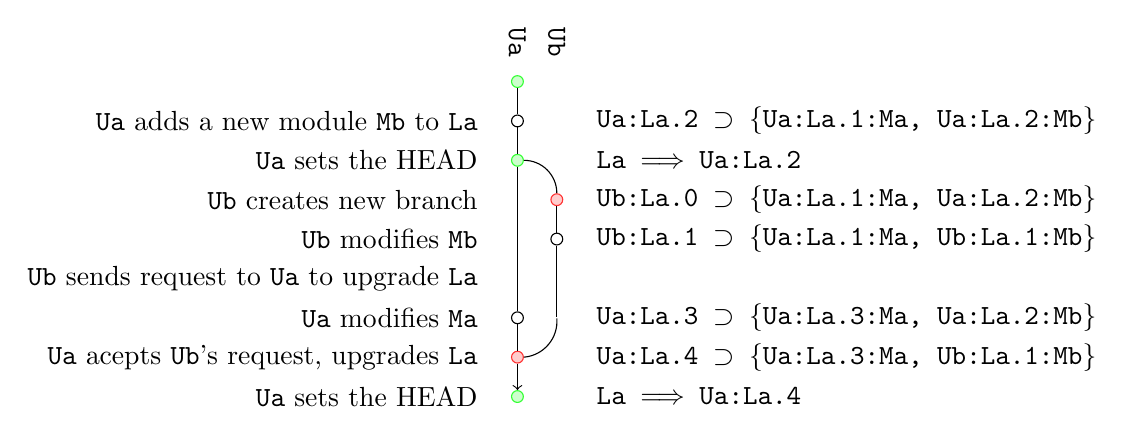
\begin{tikzpicture}[
			save/.style={circle,draw,minimum size=1.5mm},
			branch/.style={circle,draw=red!80,fill=red!20,minimum size=1.5mm},
			heads/.style={circle,draw=green!80,fill=green!20,minimum size=1.5mm},
			branchfrom/.style={circle},
			point/.style={circle,minimum size=0pt},
			labr/.style={anchor=west,font=\tt},
			labl/.style={anchor=east},
			bend angle=45,
			inner sep=0pt]
			\node at (0,5mm) [rotate=270] {\Ua};\node at (5mm,5mm) [rotate=270] {\Ub};
			\node [heads] 		(UaLa1) 		at (0,0)					{};
			\node [save]			(UaLa2)		at (0,-5mm)				{}
				edge (UaLa1)
				node [labr] at (10mm,-5mm)	{Ua:La.2 \eq \{Ua:La.1:Ma, Ua:La.2:Mb\}}
				node [labl] at (-5mm,-5mm)	{\Ua\ adds a new module \Mb\ to \La};
			\node [heads]			(LaUaLa2)		at (0,-10mm)				{}
				edge (UaLa2)
				node [labr] at (10mm,-10mm) {La \hto Ua:La.2}
				node [labl] at (-5mm,-10mm) {\Ua\ sets the HEAD};
			\node [branch]		(UbLa0)		at (5mm,-15mm)			{}
				edge [bend right] (LaUaLa2)
				node [labr] at (10mm,-15mm) {Ub:La.0 \eq \{Ua:La.1:Ma, Ua:La.2:Mb\}}
				node [labl] at (-5mm,-15mm) {\Ub\ creates new branch};
			\node [save] 			(UbLa1)		at (5mm,-20mm)			{}
				edge (UbLa0)
				node [labr] at (10mm,-20mm) {Ub:La.1 \eq \{Ua:La.1:Ma, Ub:La.1:Mb\}}
				node [labl] at (-5mm,-20mm) {\Ub\ modifies \Mb}
				node [labl] at (-5mm,-25mm) {\Ub\ sends request to \Ua\ to upgrade \La}
				node [point] (p1) at (5mm,-30mm) {} edge [-] (UbLa1);
			\node [save]			(UaLa3)		at (0,-30mm)				{}
				edge (LaUaLa2)
				node [labr] at (10mm,-30mm) {Ua:La.3 \eq \{Ua:La.3:Ma, Ua:La.2:Mb\}}
				node [labl] at (-5mm,-30mm) {\Ua\ modifies \Ma};
			\node [branch]		(UaLa4)		at (0,-35mm)				{}
				edge (UaLa3)
				edge [bend right] (p1)
				node [labr] at (10mm,-35mm) {Ua:La.4 \eq \{Ua:La.3:Ma, Ub:La.1:Mb\}}
				node [labl] at (-5mm,-35mm) {\Ua\ acepts \Ub's request, upgrades \La};
			\node [heads]			(LaUaLa4)		at (0,-40mm)				{}
				edge [<-] (UaLa4)
				node [labr] at (10mm,-40mm) {La \hto Ua:La.4}
				node [labl] at (-5mm,-40mm) {\Ua\ sets the HEAD};
		\end{tikzpicture}\vspace{4mm}

		\noindent Result: {\tt La \hto Ua:La.4 \eq \{Ua:La.3:Ma, Ub:La.1:Mb\}}

	\subsection{Scenario (2 Modules, 2 Users, no dependencies)}
	
		\Ua\ and \Ub\ are working on \La\\ 
		\Ub\ created module \Mb\
		
		\vspace{5mm}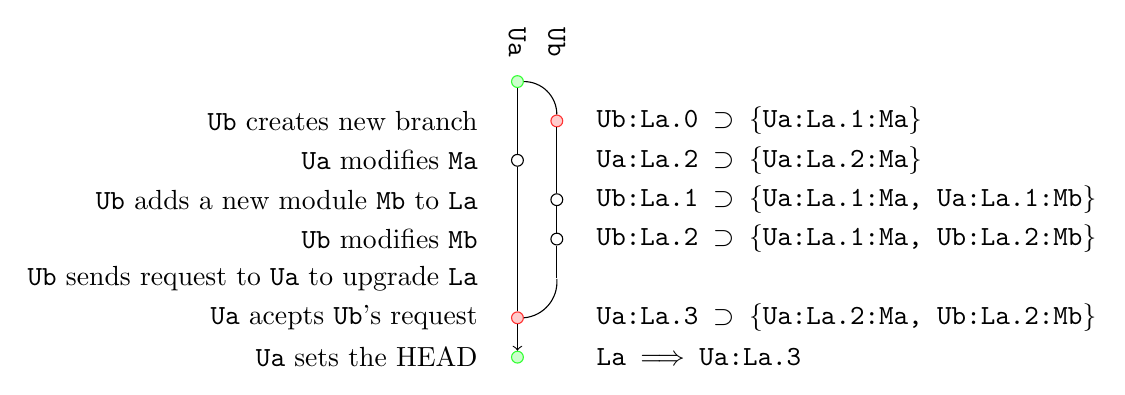
\begin{tikzpicture}[
			save/.style={circle,draw,minimum size=1.5mm},
			branch/.style={circle,draw=red!80,fill=red!20,minimum size=1.5mm},
			heads/.style={circle,draw=green!80,fill=green!20,minimum size=1.5mm},
			branchfrom/.style={circle},
			point/.style={circle,minimum size=0pt},
			labr/.style={anchor=west,font=\tt},
			labl/.style={anchor=east},
			bend angle=45,
			inner sep=0pt]
			\node at (0,5mm) [rotate=270] {\Ua};\node at (5mm,5mm) [rotate=270] {\Ub};
			\node [heads] 		(UaLa1) 		at (0,0)					{};
			\node [branch]		(UbLa0)		at (5mm,-5mm)				{}
				edge [bend right] (UaLa1)
				node [labr] at (10mm,-5mm)	{Ub:La.0 \eq \{Ua:La.1:Ma\}}
				node [labl] at (-5mm,-5mm)	{\Ub\ creates new branch};
			\node [save]			(UaLa2)		at (0,-10mm)				{}
				edge (UaLa1)
				node [labr] at (10mm,-10mm) {Ua:La.2 \eq \{Ua:La.2:Ma\}}
				node [labl] at (-5mm,-10mm) {\Ua\ modifies \Ma};
			\node [save]			(UbLa1)		at (5mm,-15mm)			{}
				edge (UbLa0)
				node [labr] at (10mm,-15mm) {Ub:La.1 \eq \{Ua:La.1:Ma, Ua:La.1:Mb\}}
				node [labl] at (-5mm,-15mm) {\Ub\ adds a new module \Mb\ to \La};
			\node [save]			(UbLa2)		at (5mm,-20mm)			{}
				edge (UbLa1)
				node [labr] at (10mm,-20mm) {Ub:La.2 \eq \{Ua:La.1:Ma, Ub:La.2:Mb\}}
				node [labl] at (-5mm,-20mm) {\Ub\ modifies \Mb}
				node [labl] at (-5mm,-25mm) {\Ub\ sends request to \Ua\ to upgrade \La}
				node [point] (p1) at (5mm,-25mm) {} edge [-] (UbLa2);
			\node [branch]		(UaLa3)		at (0,-30mm)				{}
				edge (UaLa2)
				edge [bend right] (p1)
				node [labr] at (10mm,-30mm) {Ua:La.3 \eq \{Ua:La.2:Ma, Ub:La.2:Mb\}}
				node [labl] at (-5mm,-30mm) {\Ua\ acepts \Ub's request};
			\node [heads]			(LaUaLa3)		at (0,-35mm)				{}
				edge [<-] (UaLa3)
				node [labr] at (10mm,-35mm) {La \hto Ua:La.3}
				node [labl] at (-5mm,-35mm) {\Ua\ sets the HEAD};
		\end{tikzpicture}\vspace{5mm}
		
		\noindent Result: {\tt La \hto Ua:La.3 \eq \{Ua:La.2:Ma, Ub:La.2:Mb\}}

	\subsection{Scenario with conflict (2 Modules, 2 Users, no dependencies)}

		\Ua\ and \Ub\ are working on \La\\ 
		\Ua\ created module \Mb\\
		\Ua\ and \Ub\ are working on \Mb\\
		Conflict arises...
		
		
		
		\vspace{5mm}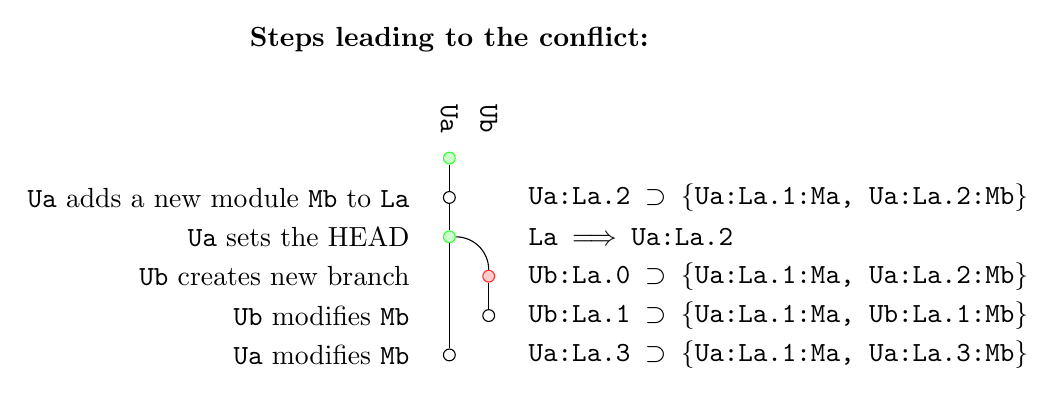
\begin{tikzpicture}[
			save/.style={circle,draw,minimum size=1.5mm},
			branch/.style={circle,draw=red!80,fill=red!20,minimum size=1.5mm},
			heads/.style={circle,draw=green!80,fill=green!20,minimum size=1.5mm},
			conflict/.style={rectangle,draw=red,fill=red,minimum size=1.5mm},
			branchfrom/.style={circle},
			point/.style={circle,minimum size=0pt},
			labr/.style={anchor=west,font=\tt},
			labl/.style={anchor=east},
			bend angle=45,
			inner sep=0pt]
			\node at (0,15mm) {\bf Steps leading to the conflict:};
			\node at (0,5mm) [rotate=270] {\Ua};\node at (5mm,5mm) [rotate=270] {\Ub};
			\node [heads] 		(UaLa1) 		at (0,0)					{};			
			\node [save]			(UaLa2)		at (0,-5mm)				{}
				edge (UaLa1)
				node [labr] at (10mm,-5mm)	{Ua:La.2 \eq \{Ua:La.1:Ma, Ua:La.2:Mb\}}
				node [labl] at (-5mm,-5mm)	{\Ua\ adds a new module \Mb\ to \La};
			\node [heads]			(LaUaLa2)		at (0,-10mm)				{}
				edge (UaLa2)
				node [labr] at (10mm,-10mm) {La \hto Ua:La.2}
				node [labl] at (-5mm,-10mm) {\Ua\ sets the HEAD};
			\node [branch]		(UbLa0)		at (5mm,-15mm)			{}
				edge [bend right] (LaUaLa2)
				node [labr] at (10mm,-15mm) {Ub:La.0 \eq \{Ua:La.1:Ma, Ua:La.2:Mb\}}
				node [labl] at (-5mm,-15mm) {\Ub\ creates new branch};
			\node [save] 			(UbLa1)		at (5mm,-20mm)			{}
				edge (UbLa0)
				node [labr] at (10mm,-20mm) {Ub:La.1 \eq \{Ua:La.1:Ma, Ub:La.1:Mb\}}
				node [labl] at (-5mm,-20mm) {\Ub\ modifies \Mb};
			\node [save] 			(UaLa3)		at (0mm,-25mm)			{}
				edge (LaUaLa2)
				node [labr] at (10mm,-25mm) {Ua:La.3 \eq \{Ua:La.1:Ma, Ua:La.3:Mb\}}
				node [labl] at (-5mm,-25mm) {\Ua\ modifies \Mb};

		\end{tikzpicture}\vspace{5mm}
		
		\noindent Libraries {\tt Ub:La.1} and {\tt Ua:La.3} are {\bf conflicted} because {\tt Ub:La.1:Mb} and 
		{\tt Ua:La.3:Mb} are both an evolution of the {\tt Ua:La.2:Mb}. From that moment many scenarios may 
		happen. Just a few of them will follow.
		
		\subsubsection{\Ua\ sets HEAD and \Ub's revision is outdated}
		
		\La's manager --- \Ua\ has chosen the HEAD. At that moment he doesn't know about \Ub's changes to \Mb.
		
		\vspace{5mm}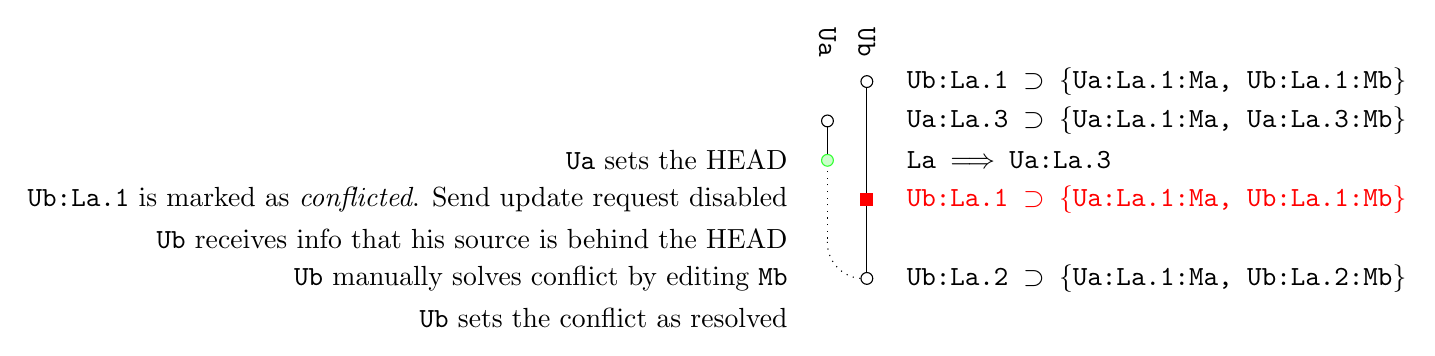
\begin{tikzpicture}[
			save/.style={circle,draw,minimum size=1.5mm},
			branch/.style={circle,draw=red!80,fill=red!20,minimum size=1.5mm},
			heads/.style={circle,draw=green!80,fill=green!20,minimum size=1.5mm},
			conflict/.style={rectangle,draw=red,fill=red,minimum size=1.5mm},
			branchfrom/.style={circle},
			point/.style={circle,minimum size=0pt},
			labr/.style={anchor=west,font=\tt},
			labl/.style={anchor=east},
			bend angle=45,
			inner sep=0pt]
			\node at (0,5mm) [rotate=270] {\Ua};\node at (5mm,5mm) [rotate=270] {\Ub};
			\node [save] 			(UbLa1)		at (5mm,0mm)			{}
				node [labr] at (10mm,-0mm) {Ub:La.1 \eq \{Ua:La.1:Ma, Ub:La.1:Mb\}};
			\node [save] 			(UaLa3)		at (0mm,-5mm)			{}
				node [labr] at (10mm,-5mm) {Ua:La.3 \eq \{Ua:La.1:Ma, Ua:La.3:Mb\}};
			\node [heads]			(LaUaLa3)		at (0,-10mm)				{}
				edge (UaLa3)
				node [labr] at (10mm,-10mm) {La \hto Ua:La.3}
				node [labl] at (-5mm,-10mm) {\Ua\ sets the HEAD}
				node [point] (p1) at (0,-20mm) {}
				edge [dotted] (LaUaLa3);
			\node [conflict] 		(CUbLa1)		at (5mm,-15mm)			{}
				edge (UbLa1)
				node [labl] at (-5mm,-15mm) {{\tt Ub:La.1} is marked as {\em conflicted}. Send update 
										request disabled}
				node [labl] at (-5mm,-20mm) {\Ub\ receives info that his source is behind the HEAD}
				node [labr,red] at (1cm,-15mm) {Ub:La.1 \eq \{Ua:La.1:Ma, Ub:La.1:Mb\}};
			\node [save]			(UbLa2)		at (5mm,-25mm)			{}
				edge (CUbLa1)
				edge [dotted, bend left] (p1)
				node [labr] at (1cm,-25mm) {Ub:La.2 \eq \{Ua:La.1:Ma, Ub:La.2:Mb\}}
				node [labl] at (-5mm,-25mm) {\Ub\ manually solves conflict by editing \Mb}
				node [labl] at (-5mm,-30mm) {\Ub\ sets the conflict as resolved};
		\end{tikzpicture}\vspace{5mm}
		
		From that moment {\Ub:La.2} becomes a normal (not conflicted) PackageRevision. \Ub\ may send
		Package manager an upgrade request which could end by switching \La's HEAD to {\Ub:La.2}.
		It is important to note, that the {\tt Ub:La.2} is not an evolution of {\tt Ua:La.3}, it will not be
		originated from it.\footnote{Decide if this is the right thing to do.}

		\subsubsection{\Ub\ sends update request, \Ua\ decides to drop his changes}
		
		\Ub\ thinks his change to \Mb\ is finished and requests update of the Library from its manager --- \Ua.
		He accepts the request and marks his version of this module as discontinued. This mark prevents from 
		the automatic set to conflicted revision.
		
		\vspace{5mm}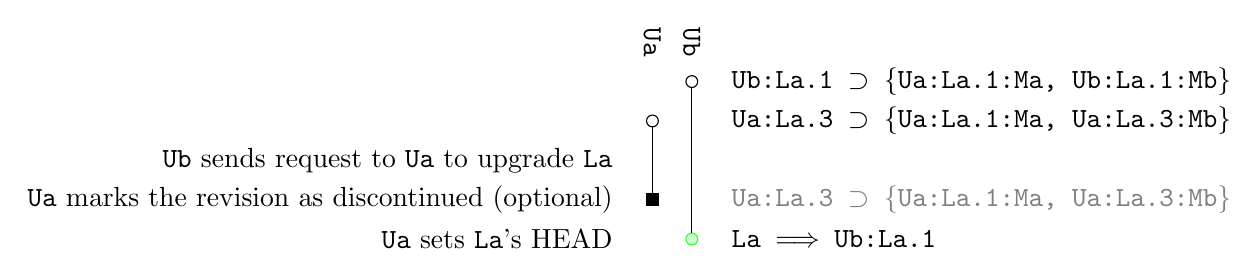
\begin{tikzpicture}[
			save/.style={circle,draw,minimum size=1.5mm},
			branch/.style={circle,draw=red!80,fill=red!20,minimum size=1.5mm},
			heads/.style={circle,draw=green!80,fill=green!20,minimum size=1.5mm},
			conflict/.style={rectangle,draw=red,fill=red,minimum size=1.5mm},
			discontinued/.style={rectangle,draw=black,fill=black,minimum size=1.5mm},
			branchfrom/.style={circle},
			point/.style={circle,minimum size=0pt},
			labr/.style={anchor=west,font=\tt},
			labl/.style={anchor=east},
			bend angle=45,
			inner sep=0pt]
			\node at (0,5mm) [rotate=270] {\Ua};\node at (5mm,5mm) [rotate=270] {\Ub};
			\node [save] 			(UbLa1)		at (5mm,0mm)			{}
				node [labr] at (10mm,-0mm) {Ub:La.1 \eq \{Ua:La.1:Ma, Ub:La.1:Mb\}};
			\node [save] 			(UaLa3)		at (0mm,-5mm)			{}
				node [labr] at (10mm,-5mm) {Ua:La.3 \eq \{Ua:La.1:Ma, Ua:La.3:Mb\}};
			\node [labl] at (-5mm,-10mm) {\Ub\ sends request to \Ua\ to upgrade \La};
			\node [discontinued] 	(DUaLa3)		at (0,-15mm)			{}
				edge (UaLa3)
				node [labl] at (-5mm,-15mm) {\Ua\ marks the revision as discontinued (optional)}
				node [labr,gray] at (1cm,-15mm) {{Ua:La.3 \eq \{Ua:La.1:Ma, Ua:La.3:Mb\}}};
			\node [heads]		(LaUbLa1)		at (5mm,-20mm)			{}
				edge (UbLa1)
				node [labr] at (1cm,-2cm) {La \hto Ub:La.1}
				node [labl] at (-5mm,-2cm) {\Ua\ sets \La's HEAD};
					
		\end{tikzpicture}\vspace{5mm}

\section*{Draft/Ideas}
	\begin{description}
		\item[update Library] if Library HEAD has been changed something should tell the User that an update 
		is possible. It should then (on request) change the versions of all Modules which are not in conflict 
		with updating Library. In essence, if \\
			{\tt Ua:La.1 \eq \{Ua:La.1:Ma, Ub:La.2:Mb\}} is a Library to be updated and \\
			{\tt La \hto Uc:La.3 \eq \{Ub:La.1:Ma, Uc:La.3:Mb, Uc:La.1:Mc\}} is current HEAD, then\\
			{\tt Ub:La.2:Mb} should be updated to {\tt Uc:La.3:Mb} and {\tt Uc:La.1:Mc} should be added.\\
			User should receive a notification that {\tt Ua:La.1:Ma} is not in sync with HEAD.
	\end{description}

\section*{To be continued\ldots}
\end{document}

